\section{The `Calibrate' option}\seclab{Calibration}

This option is used to perform the time-calibration of all antennas and antenna stations.

The calibration is run from the script \verb!"Calibrate.sh"! where the input is set in the file \verb!"Calibrate.in"!. The calibration script has to be run many times over, first to obtain sources of sufficient quality (stand alone, little interference with others, similar structure for all antennas, visible in even and odd numbered antennas) using calibration files from another flash, followed by runs where the antenna calibration is fixed at the nanosecond level.  The scripts need to be run in the FlashFolder.

The general philosophy is to select a few of the strongest pulses in different parts of the lightning discharge. These should cover the spatial extent of the flash reasonably well. The exploration map, see \secref{Explore}, is a good tool to select times at which to search for the good sources for time calibration.
Pulses located in a few independently selected chunks of data on the reference antenna should be fitted simultaneously, i.e.\ fitting simultaneously all source locations as well as station and antenna timings.

The different steps in calibration are
\begin{enumerate}
\item Find calibration source that are spread reasonably homogeneously over the complete extent of the storm.
\begin{enumerate}
\item Either from 'Explore.out' or from 'Img\_Explore.pdf' find the times for which the active regions in the storm covers all areas.
\item For each of these times run the imager (using the calibration from another flash) for a time span of -not more- than 1~ms with an input line like
{
\tiny \begin{verbatim}
   948  , 11900.  -26204.    5950.   , 0 1.
\end{verbatim}
}
and it will generate a file named 'Srcs22-5star-$\cdots$.dat'.
\item Cut a section from this 5star file that resembles

\begin{linenumbers}
\tiny
\resetlinenumber
\begin{verbatim}
    974.771040      15.70      -1.85       7.53  4479001
C 2 2 1   38719  10064.73,  -5428.98,  11197.11,     0.97491;    0.417,  0.7154,  0.4560,  0.8930,  31,  38,   3361,  8, 10,  0
C 9 2 1   40061  15720.37,  -1856.59,   7545.11,     0.97491;   23.390, 19.5381, 10.0996,  9.3094,  31,  38,   1423,  9, 10,  0
C 1 2 1   15254  15550.96,  -1838.29,   7466.56,     0.97479;    4.493,  0.1831,  0.3413,  0.6994,  30,  30,   5921,  6, 15,  1
C 8 2 1   39836  15515.73,  -1860.96,   7448.69,     0.97491;   13.274, 15.2286,  7.8900,  7.4356,  25,  30,   1549, 10,  6,  1
\end{verbatim}
\end{linenumbers}
and paste this in the input of 'Calibrate.in' which should now look like what is shown in \secref{Fcal}. Make sure that the location specifies in the chunk line (starting at t=974.771040~ms for this case) is pointing to the right general direction. The coordinates of (N,E,h) may all three be specified in units of m or km, whichever you prefer.
\item At this stage I found it more efficient to work on each chunk separately.
\item Check the generated curtain plots carefully. 1) Make sure the pulse in the reference station is reasonably well separated from others and is not wide. 2) The pulse is seen in even and odd antennas. 3) mark for exclusion those stations for which the pulse differs from what is seen in the reference antenna. The resulting input should resemble what in given is \secref{Scal}.
\item Run the case of \secref{Scal} a few times until the chi-square per degree of freedom for each source (as listed at the end of the 'Calibrate.out' file) is reasonable, typically below 5 or 10. When there are sources that are notoriously bad, omit them from the calculation. It may be useful to check .out file for the contributions of each station to the chi-square of each source. Listed are the mean time difference and the standard timing error for a station. If one of these is large, check the curtain plot for the reason and use this to base your decision to mark a station for exclusion.
\item Repeat these steps for a few different chunks until you have covered the complete extent of the storm.
\end{enumerate}
\item Combine all calibration sources in one calibration run, where each chunk line is followed by lines with the sources and excluded antennas. The input should resemble what is given in \secref{Scal}.
\item Run this while fitting all station timings as well as source locations as specified by the line
{
 \tiny \begin{verbatim}
abut  !
\end{verbatim}
}
where there should be no leading spaces. In the namelist set ' WriteCalib=.true. ,' and possibly ' FitRange\_Samples=10 ,'. On the basis of the result you may want to exclude (or include again) some stations, but always consult the curtain plots. If so, re-run. Always copy the chunk and source lines at the end of the .out file into the .in file and cut and paste the calibration line into the namelist of the .in file.
\item Next is to fit the antenna timings within a station. To do so replace the 'abut' line with
{
\tiny \begin{verbatim}
antenna RS106 RS205 RS208 CS301  RS306 RS307 RS310 RS406 RS409 CS501 RS508 RS509 NoSrc !
\end{verbatim}
}
where you list the stations for which the antenna timings could use adjustment. Experience tells that about 12 stations is the max the program can handle when using 'NoSrc', specifying that the parameters of the sources are not varied during the search. The program will protest if the number is too large.
\item Repeat this for all stations. Cut and paste the name of the generated .cal file to the input for the next run.
\item After adjusting the timings of the antennas within each station, the timing standard deviation per station and per source should be order 1~ns or less. To guarantee this (and allow some lee-way put ' StStdDevMax\_ns=2. ,' in the namelist input. This will mark for exclusion all stations for which this value is exceeded. Probably repeat the antenna calibration runs.
\item Check in the process that for each station there are a sufficient number, typically 5) of calibration sources left (for each orientation). If the number is smaller, either find more possible calibration sources (i.e. go to the beginning of this recipe) or exclude the station from the analysis (and later imaging). This may happen if the station is at a too large distance from the source region and thus has a -comparatively- high noise level.
\item Use again the option 'abut !' to make a final station timing and calibration source adjustment.
\end{enumerate}

Added notes:
\\1) It is more efficient to replace step 1b by en earlier imaging of the complete flash with an approximate calibration and to select for step 1c the appropriate parts of the long 5star file that was generated in the imaging of the complete flash. Note that the generated image is probably poor (do use ' AntennaRange=100').
\\2) In step 1d care should be taken that at the end of the procedure a pulse is seen (or is likely hidden in the noise) for all antennas (even if they are too noisy or messy to include in the calibration) at the expected position. If not this implies that the source location must be off and thus this peak will not contribute to a reliable calibration. To steer the source-position search play a bit with 'FitRange\_Samples' since this variable sets the range from the expected position where pulses may be included in the search. It requires some trial-and-error to get a 'feel' for this variable. Its value is very important so pay attention!


\subsection{First calibration stage}\seclab{Fcal}

For the first run the typical content of \verb!"Calibrate.in"! is like

\begin{linenumbers}
\tiny
\resetlinenumber
\begin{verbatim}
&Parameters
 RunOption='Callibrate'
 CurtainHalfWidth=100  !
! XcorelationPlot=.true. ,
! FullAntFitPrn=.true.
 AntennaRange=100
 FitRange_Samples=20
 SaturatedSamplesMax=3 ,
 StStdDevMax_ns=20. ,
! WriteCalib=.true.
!  Calibrations="Hil21C-3-202204260923.cal" ! Hilbert T  1.44 antenna
  Calibrations="Hil21C-2-202204262256.cal" ! Hilbert T  6.48
 SignFlp_SAI=  142092, 142093
 PolFlp_SAI=  32086,
 BadAnt_SAI=   003065, 021078, 021079, 021093, 026030, 32016, 32017, 32048, 32049,
               101045, 125029, 150065, 188051, 188094, 188095
! OutFileLabel="T"
&end

    974.771040      15.70      -1.85       7.53  4479001
C 2 2 1   38719  10064.73,  -5428.98,  11197.11,     0.97491;    0.417,  0.7154,  0.4560,  0.8930,  31,  38,   3361,  8, 10,  0
C 9 2 1   40061  15720.37,  -1856.59,   7545.11,     0.97491;   23.390, 19.5381, 10.0996,  9.3094,  31,  38,   1423,  9, 10,  0
C 1 2 1   15254  15550.96,  -1838.29,   7466.56,     0.97479;    4.493,  0.1831,  0.3413,  0.6994,  30,  30,   5921,  6, 15,  1
C 8 2 1   39836  15515.73,  -1860.96,   7448.69,     0.97491;   13.274, 15.2286,  7.8900,  7.4356,  25,  30,   1549, 10,  6,  1
- - - - -- - - -- -
only !
\end{verbatim}
\end{linenumbers}

The order of the parameters in the namelist input is arbitrary. All input on the line after an exclamation sign (!) is ignored and may be used for comments, or storing parameter one may want to use on some other run. Some of the parameters were explained already and the new ones (labeled by line number) are:
\begin{enumerate}
\item[3] \verb#"! CurtainHalfWidth=100"#: curtain plots (see \secref{CurtainPlot}) are made for each calibration source with the specified width (in time samples of 5~ns). No plots are made when the width is zero or negative (default).
\item[4] \verb#"! XcorelationPlot=.true."#: No plots of the cross correlations (see \secref{XCorPlot}) are made since the default for this variable is .false..
\item[5] \verb#"! FullAntFitPrn=.true."#: No extensive printout giving the time offsets per antenna per source (see \secref{PrintOut}) is made since the default for this variable is .false..
%\item[6] \verb#"! FitIncremental=.false."#: Since the default for this variable is .true. antennas within an increasing range around the core will be included in the source locating fits, where the source locations of the previous fit are used as the guess locations for the following iterative fit in which more distant antennas are included.
\item[6] \verb#" AntennaRange=100"#: All antennas within a distance of 100~km from the core will be included in the calculations.
\item[7] \verb#" FitRange_Samples=20"#: The maximal range, in samples (of 5 ns), that is searched for a pulse around the predicted location (based on the pulse location guess). The range may be made smaller if the error on the guess location is small. In a first run the value for \verb!FitRange_Samples! should be relatively large to be able to find peaks also for antennas that are very poorly calibrated. Later in the calibration process it will be tuned down.
%\item[8] \verb!" Dual=.false."!: The peaks in even and odd numbered antennas will be searched for independently. In a later round the two will be coupled.
\item[8] \verb#" SaturatedSamplesMax=3"#:  Maximum number of saturates time samples per chunk of data. 3 may be a bit conservative.
\item[9] \verb#"! StStdDevMax_ns= 20 "#:  Stations are excluded when the standard deviation in antenna-arrival times for a pulse in one station exceeds this value.
\item[10] \verb#"! WriteCalib=.true."#: The obtained new antenna calibrations (if calculated) will not be written to an updated calibration-data file.
\item[20] \verb#"      974.771040      15.70      -1.85       7.53  "#: A chunk-specification line. In this example a single one, but the number is free. It specifies the time-slots where pulses should be searched as well as the general expected location of the sources. Separating commas are not necessary. These times and locations are obtained from the earlier Explore run. It is recommended to stay below 5 entries. The experience is that it is easier to try different sections of the flash in separate runs.
    \begin{description}
    \item[974.771040] The data chunk of 0.3~ms length starting at this time (in [ms]) will be used.
    \item[15.70      -1.85       7.53] The position (N,E,h)  that is taken as a first guess for the source positions (specified in either [m] or [km], a mix is not allowed). The location should be in the right quadrant, but not more precise. Note that the first character on the line should not be left as a space.
    \end{description}
\item[21 $\cdots$ 24] \verb#"C 9 2 1   40061  15720.37,  -1856.59,   7545.11, "#: Specification of the peaks that should be considered. For this example this line was cut\&paste from 'Srcs22-5star-.dat', which appears more efficient. The lines can also be omitted and some candidate sources will be searched. Note that the formatting of this line is very important.
    \begin{description}
    \item[C] the sample number of the peak is given as if the antenna were right at the core.
    \item[ 9] The 9$^{th}$ pulse as found by the imager. This number is not used, but may be good for your own bookkeeping.
    \item[ 2] The same source is used for even and odd numbered antennas. Note that all should be labeled with with '2' or none, no checking is done. Alternatively it is possible to specify even ('0') and odd ('1') antennas separately, see \secref{Scal}.
    \item[ 1] The chunk number.
    \item[ 40061] The sample number specifying the location of the peak on the time trace.
    \item[15720.37,  -1856.59,   7545.11] The position (N,E,h) in [m] that is taken as a good guess for the source position.
    \end{description}
\item[25] \verb#" - - - - -- - - -- - "#: A closing line as long as it does not contain a line with number, but only text.
\item[26] \verb#"only !"#: No search for antenna calibrations is done at this stage, source locations only.
\end{enumerate}

Running the script \verb!"Calibrate.sh"! for this input file goes fast and will crate the files  \verb!"Calibrate.out"! with much diagnostics concerning the fit results for all sources as well as a series of plots, see \secref{Cal-out}.

\subsubsection{Discussion}

In calibrating one should use the stronger sources (seen in more antennas), narrow pulses (better timing resolution since extended sources have some intrinsic resolution), and pulses that are in a rather low-noise background (few other pulses in the vicinity, sine these may confuse the pulse-location algorithm). To find such sources one may use  the automatic pulse-finding algorithm is used to locate the strongest pulses in each to the blocks of data (chunks in the language of LOFLI) starting at the times specified in the lines following the namelist input (starting with \verb!"&Parameters"! and ending with \verb!"&end"!). Any empty lines are skipped. The namelist input specifies the values of pre-defined control parameters where a complete list is given in \tabref{LOFLI-namelist}. A more robust procedure appears to run the imager (as described at the start of the section) with a reasonable time calibration for a very short time-span. strongest pulses that obey certain quality criteria will be written to the file 'Srcs22-5star-.dat' in a format that is suitable for cut\&paste to the input. Select the ones where for a chunk most candidates are given.

If using the -not preferred- automatic pulse-finding algorithm one should follow the following scheme to find candidate source locations.
The antennas are limited to those within a range of \verb!AntennaRange=5!~km from the core since the experience is that usually, due to non-optimal calibration, the fitting procedure starts to derail for antennas at larger distances, making the results useless. It is a matter of trial and error to learn what is best for this particular flash. To learn what was going on the output or this run, \verb!"Calibrate.out"!, should be scrutinized to find the sources and their deviations. At this stage one should pay particular attention to stations that show a large deviation. These need to be excluded (for all sources or for particular sources) for the time being (see following sections). It is in this respect also instructive to inspect the produced plots (all of them, quite a number) showing the shape of the cross correlation for each used antenna. This generally shows in the blink of an eye what went on during fitting.

If all spectra look crazy, decrease \verb!AntennaRange! and try again. If the results are reasonable, you may want to increase the value or proceed.

For a limited value for \verb!AntennaRange! sources positions for many of the pulses have been found. The source locations are not very reliable yet, but the peak in the cross correlation for these sources looks healthy (for you to judge!). The objective of this stage is to obtain the station-timing calibrations. Antenna timings will be dealt with in the last, third, stage. All good things come in three!

At this second stage the automatic pulse finding is by-passed and the locations of the pulses in the reference antennas (one for even and one for odd polarization) is specified explicitly as well as a first guess for their location. A typical content of \verb!"Calibrate.in"! is

\subsection{Second calibration stage}\seclab{Scal}

At this second stage the locations of the pulses in the reference antennas (one for even and one for odd polarization) is specified explicitly as well as a first guess for their location. A typical content of \verb!"Calibrate.in"! is

\begin{linenumbers}
\resetlinenumber
\begin{verbatim}
&Parameters
 RunOption='Calibrate'
 CurtainHalfWidth=100
 XcorelationPlot=.true. ,
! FullAntFitPrn=.true.
 AntennaRange=100
 FitRange_Samples=20
 SaturatedSamplesMax=3 ,
 StStdDevMax_ns=20. ,
 WriteCalib=.true.
!  Calibrations="Hil21C-3-202204260923.cal" ! Hilbert T  1.44 antenna
  Calibrations="Hil21C-2-202204262256.cal" ! Hilbert T  6.48
 SignFlp_SAI=  142092, 142093
 PolFlp_SAI=  32086,
 BadAnt_SAI=   003065, 021078, 021079, 021093, 026030, 32016, 32017, 32048, 32049,
               101045, 125029, 150065, 188051, 188094, 188095
! OutFileLabel="T"
&end

        900.653040     0.966    -0.871     0.122        1
C 1 0 1   14421  12017.57, -24849.06,   6785.18,   900.63029;   1.36,   1.48 RS310 RS406 RS409 RS508 RS509
exclude   RS310 RS406 RS409 RS508 RS509
C 2 1 1   14421  12017.57, -24849.06,   6785.18,   900.63029;   1.10,   1.21 RS310 RS406 RS409 RS508 RS509
exclude   CS007 RS306 RS310 RS406 RS409 RS508 RS509
        858.435360    14.520   -26.520    10.800        2
C 3 0 2   21657  14553.98, -26533.40,  10719.00,   858.43653;   2.16,   2.16
exclude   RS310 RS406 RS409 RS509
C 4 0 2   49807  14355.98, -26558.04,  10734.18,   858.57750;   2.61,   2.66 RS208
exclude   RS106 RS205 RS208 RS306 RS307 RS310 RS406 RS409 RS509
C 5 1 2   21657  14553.98, -26533.40,  10719.00,   858.43653;   2.53,   2.53
exclude   RS306 RS307 RS406 CS501
C 6 1 2   49807  14355.98, -26558.04,  10734.18,   858.57750;   1.84,   1.94 RS310 RS508 RS509
exclude   CS007 RS306 RS307 RS310 RS406 RS508 RS509
        858.653040    15.010   -27.360    11.070        3
C 7 0 3   27568  14523.43, -26508.51,  10778.41,   858.68382;   1.37,   1.46 RS310 RS409 RS508 RS509
exclude   RS208 RS310 RS406 RS409 RS508 RS509
C 8 1 3   27568  14523.43, -26508.51,  10778.41,   858.68382;   1.00,   1.08 RS310 RS409 RS508 RS509
exclude   RS306 RS307 RS310 RS406 RS409 RS508 RS509

- - - - -- - - -- -
only !
\end{verbatim}
\end{linenumbers}

The preamble, the namelist input, as well as the specification of the data-blocks (chunks in the language of LOFLI) is similar to what was used earlier, however now a list of pulses is given. This pulse information is (mostly) cut-and-paste from \verb!"Calibrate.out"!, so don't worry about typing, however the formatting, i.e.\ spaces and so, is important.

Obsolete: \verb!FitIncremental=.false.! is important at this stage. All stations within a distance of, say \verb!AntennaRange=70! [km] are taken into account where the cross correlations are calculated over an interval of \verb!FitRange_Samples=50! [samples]. The precise values for these parameters is again a matter of trial and error. At the end of this stage you want to reach \verb!AntennaRange=100! and \verb!FitRange_Samples=20! while starting with the values from the first stage, see \secref{Fcal}.

Obsolete: In this stage it is recommended to use \verb!Dual = .true.! to combine the calibrations for odd and even polarizations. With this option the sources for pulses allocated to the same sample numbers in the even and odd polarized reference antennas are taken identical.

Default is that the same pulse locations are specified for both types of antennas. Their source locations will then be tied automatically. Two separate entries for th two antenna orientations is useful at this stage since the pulses of a source do not show with equal strength and thus may require exclusion of different stations.

A new and updated calibration table will be produced with \verb!WriteCalib=.true.! while the old one remains. In the output \verb!"Calibrate.out"!, towards the end, you will find the name. If the result from this run gains your approval, you can used the updated table for a following run by specifying its name as in \verb!Calibrations= "Hil21C-2-202204262256.cal"!, for example.

The important new ingredient here is the list of pulse positions, source locations and stations that are excluded for a particular source. An undetermined number of lines is being read until there is a clash in format. The line \verb!"- - - - -- - - -- -"! does so. A line starting with single or double digits gives for each pulse in order:
\\0) first column, if `C' the pulse position (in samples) is specified as if the reference antenna is exactly at the core, other wise, the sample number for the reference antenna at its actual position, which is usually a few samples different from the center of the core.
\\1) A sequential number (ignored on read in).
\\2) The polarity (0 or 1). For each chunk  polarity 0 sources are followed by polarity 1 sources.
\\3) The chunk number (1,2, or 3 in the present case). Sources should be ordered according to chunk number.
\\4) The sample number for the pulse location in the reference antenna (integer).
\\5) The coordinates for the source location as (N,E,h).
\\The remainder of this line is ignored upon reading. The line may be followed by a line starting with \verb!"exclude"! listing the stations that should not be taken into account for this source when fitting.
\\When  \verb!Dual = .true.!, the default option, two pulses in the same chunk having the same sample number are treated as coming from the same source location during fitting. For these lines the spaces matter! With cut-and-paste this section in the right format can be obtained from the output (.out) file.

The first line following \verb!"- - - - -- - - -- -"! specifies which station timings should be searched for. Option {\bf 'only'} implies what you would guess. the list is closed with an exclamation mark. The option {\bf 'abut'} (standing for 'all but') also does what you think it should do when you have deciphered the meaning. Option {\bf `antenna'} specifies that the optimal timing calibration for the each antenna for the specified stations will be searched. Note that the options are case sensitive and should not be preceded by a space. An example is \verb!" RS509 "! where, in stead of a station, also  \verb!" NoSrc r"! can be given is the source locations should not be optimized and only antenna timings.

All remaining lines are ignored. An excellent place to store reminders or potentially useful input lines.

\subsubsection{Discussion}\seclab{D-Scal}

The objective at this stage is to use several excellent-quality sources, spread over a large volume of a flash, to calibrate the station timing. The reasoning is that over the duration of the flash all pulses in a single antenna will have the same time-shift due to calibration errors, leaving their relative arrival times unchanged. By fitting the location of sources distributed over a large volume, the relative arrival times are sufficient to fix their positions. The arrival times thus fix the antenna calibrations.

To obtain the source positions we use the fact that the relative timing for antennas in a single station have an accuracy of better than 5~ns. Also the relative timing of the core stations is known to this level. At the end we do want to improve on this, however.

The source locations found for an inner circle of antennas will yield a prediction when the pulses arrive in the antennas in the next circle out losing accuracy for larger distances. Thus by increasing \verb!AntennaRange! by not too much the pulse is likely to lie in the next ring of antennas at the predicted time within \verb!FitRange_Samples! and will thus be located in the search algorithm. If the pulse is further away, it will not be located in this particular antenna. In other antennas the situation might be better, and thus the obtained source position is improved, while this particular antenna, for this particular pulse is marked as 'excluded' in the output. In a next round with the same settings, but updated source locations, the pulse may be found. This indicates the delicate balance between the various variables.

At all stages it is VERY STRONGLY recommended to look at the curtain, see \secref{CurtainPlot}, and the cross-correlation, see  \secref{XCorPlot}, plots to decide if a station should continue to be excluded, or was included while the cross correlation was a mess. At the end one prefers to have a minimal number of excluded stations.

During this process it is recommended to perform an intermediate calibration of (some of) the station timing, using the options only or abut. This will stabilize the results for following rounds.

The output file \verb!"Calibrate.out"! contains a part that resembles the sample input. Certainly after each calibration table update the source locations should be updated, but it is better to do so more frequently.

Occasionally you may find that when making curtainplots, see \secref{CurtainPlots} one station or even one antenna is completely off. In such a case the calibration file should be edited to correct this (it should be self evident what to do). Once the offset is reduced to less than \verb!FitRange_Samples! the program can be used to reduce the error.

At the end of the day all station should be involved in the fitting process with at least ten sources distributed over the flash with an RMS error of about 2~ns. During the fitting process the error assigned to the extracted peak in the correlation spectrum is 1~ns.

Do not despair, after a few weeks of struggling you are sure to have some vague idea of the logic behind this procedure.

\subsection{Third calibration stage}

In the third calibration stage the individual antennas will be calibrated. The same procedure will be followed as for the second stage, only now option {\bf `antenna'} is set replacing the `only' in the list of stations that are to be fitted. Since fitting all antennas simultaneously requires too much memory, this is done in different batches. At the end of the day a $\chi^2$ of order unity should be obtained, or an RMS deviation of 1~ns.

\subsection{Figures and print-out}\seclab{Cal-out}

\subsubsection{Curtain plot}\seclab{CurtainPlot}

When you feel completely lost (but also if you are not), it is instructive to switch on \\\verb! CurtainHalfWidth=100 ! to make a -so named- curtain plot showing the spectra for all antennas, sorted per peak (sorry, only for peaks listed for the even numbered antennas) and separate for even and odd antenna numbers. In this case 100 gives the half-width of the time-window, the number of time samples before and after the lined-up part, that will be shown in the figures

Many figures named like \verb!"CuP-02.pdf"! will be created showing all spectra where the antenna timings are adjusted such that if these pulses indeed comes from a source at the position of source \#02, all peaks would be lined-up perfectly, see \figref{Cal-Curtain}. The time traces for the same station and polarity are overlayed.

\begin{figure}[th]
\centering{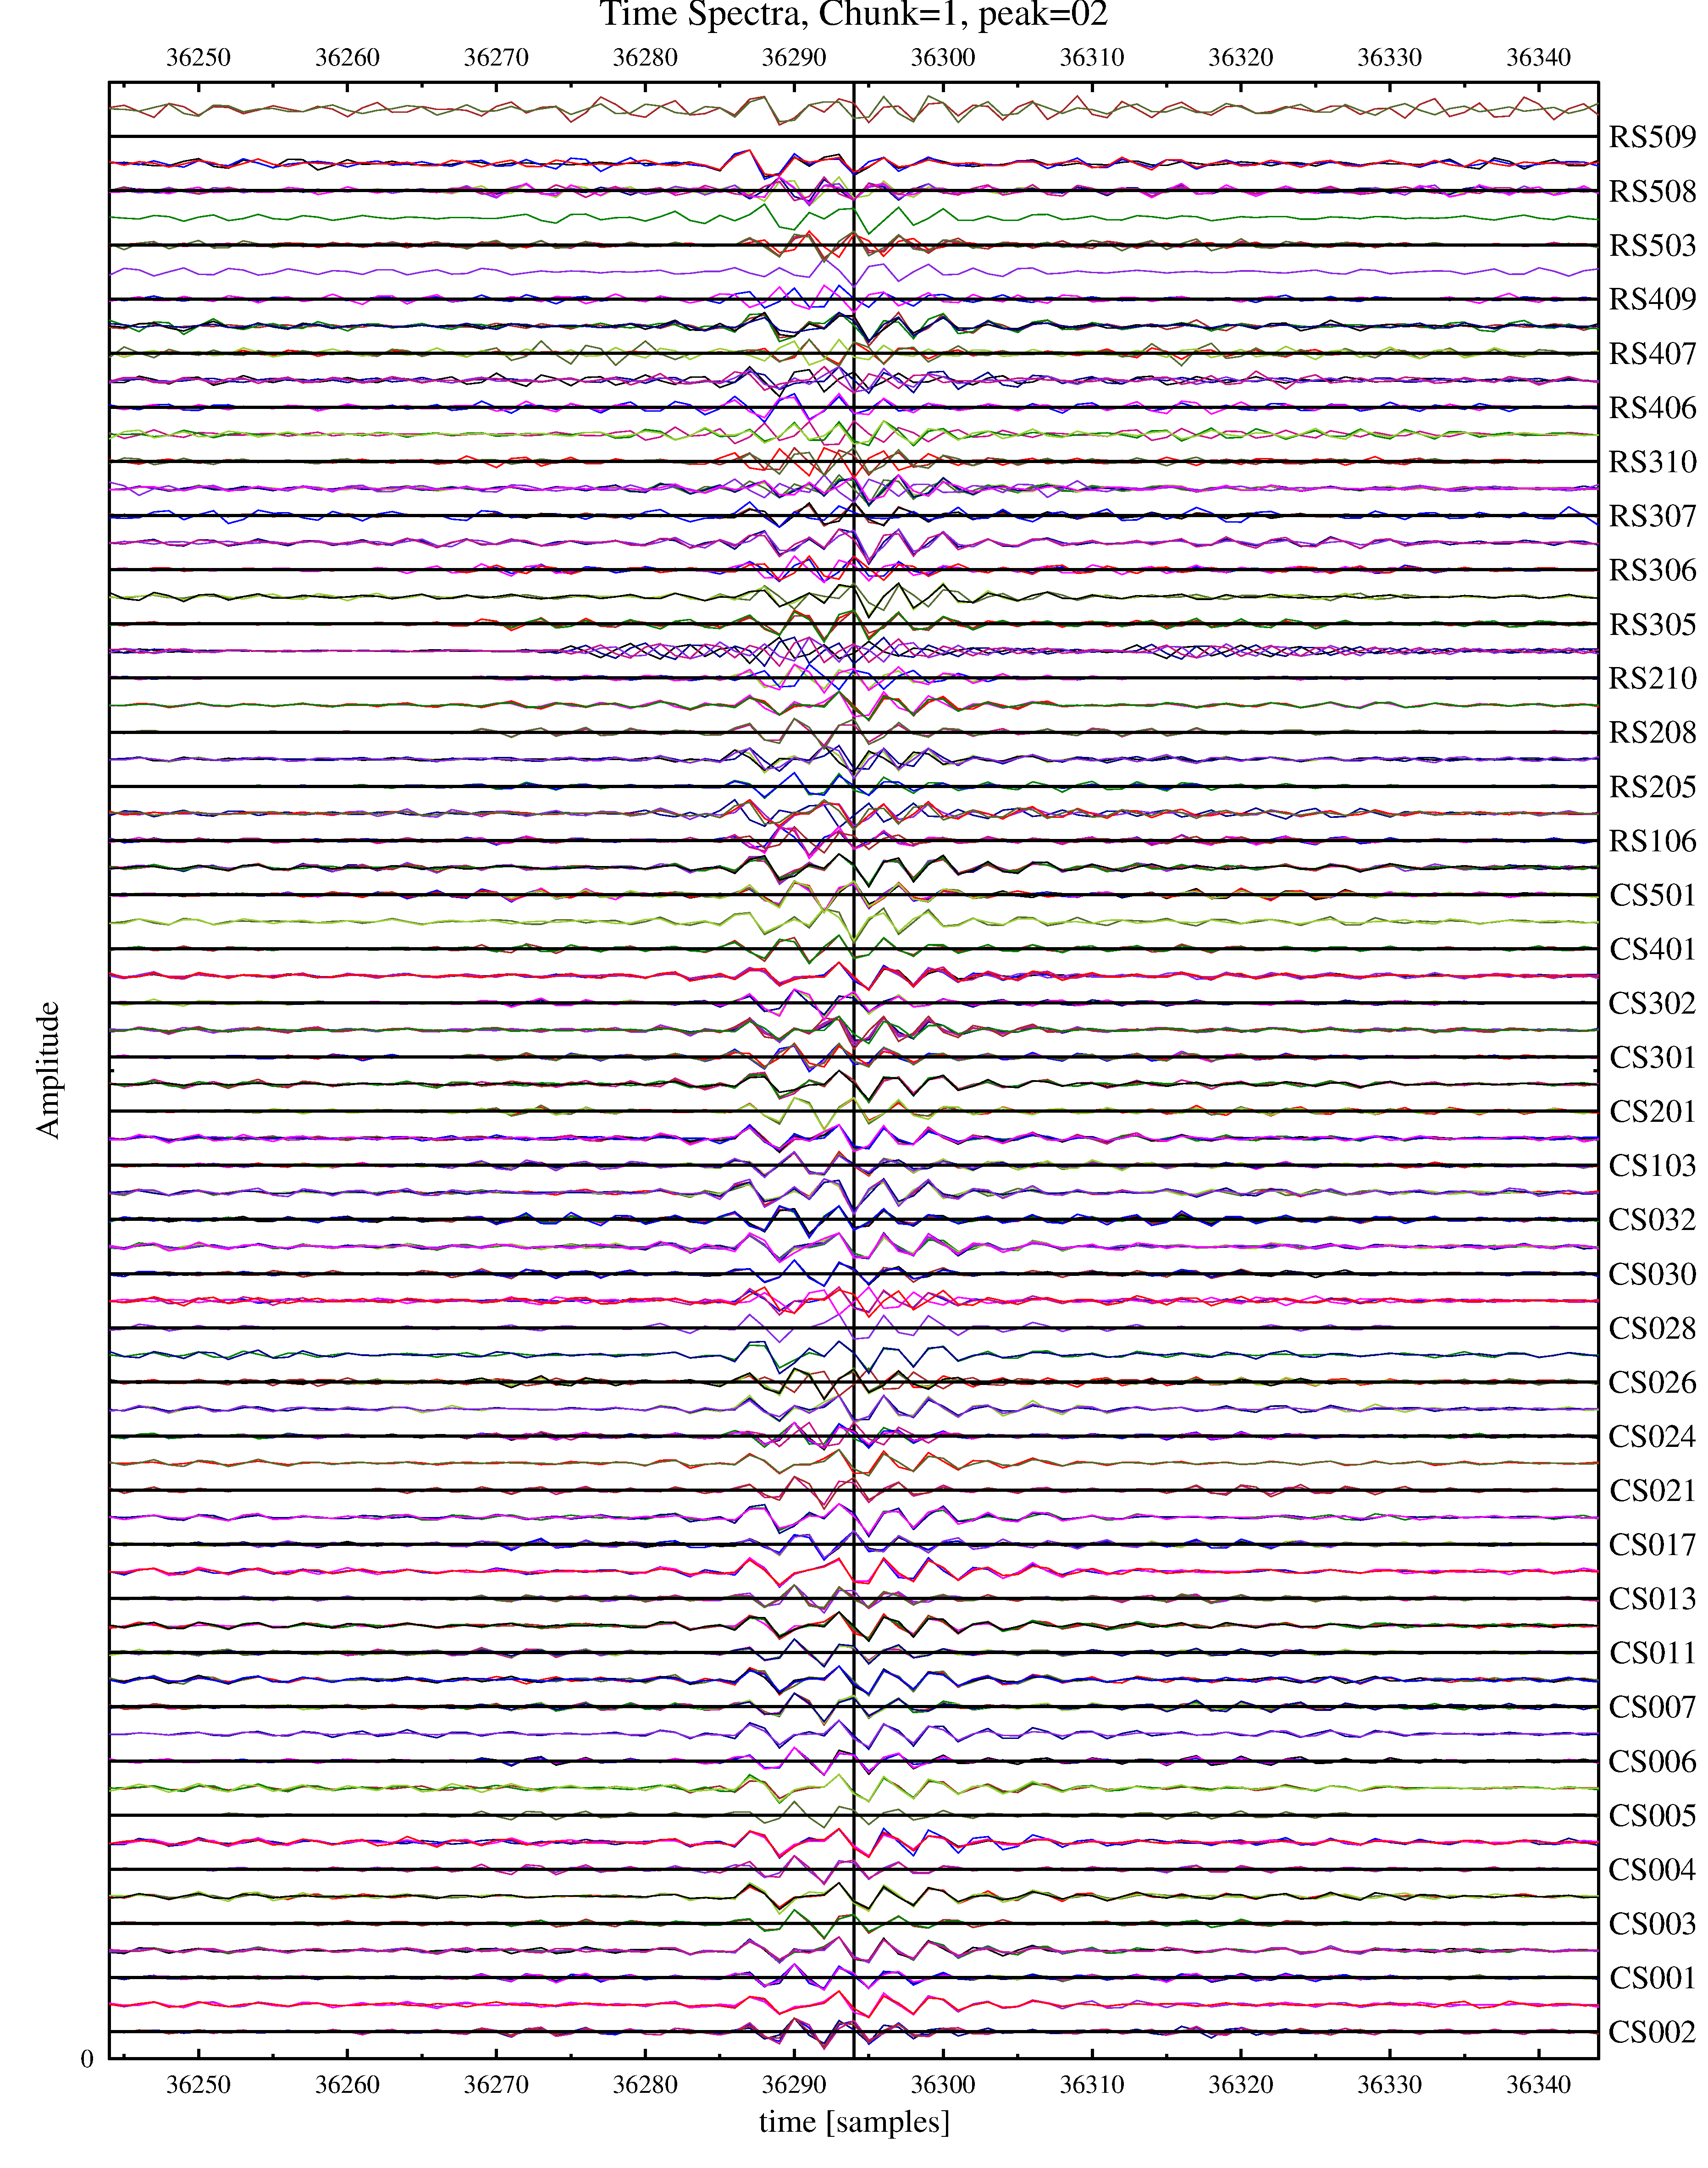
\includegraphics[width=0.59\textwidth]{Figs/CuP-02-18D1} }
%\centering{\includegraphics[ bb=1.0cm 2.4cm 24.5cm 25.7cm,clip, width=0.49\textwidth]{../Figs/SE20A7-NPMx_1HIntfSpecSel} }
	\caption{A curtain plot for the second source for a typical flash.}	 \figlab{Cal-Curtain}
\end{figure}

The pulses in all antennas can be included in the calibration calculation if the pulses line-up nicely. To see this better the time-window can be adjusted. The pulse amplitudes have been normalized for each spectrum to the maximum, say unity.
\\The structure of the pulses in all odd numbered antennas should resemble each other. The same for the even numbered antennas. The pulse for in the odd may be different from that in the even ones.
\\The noise level should hardly be visible on the plotted scale.
\\If one condition is not obeyed the antenna should be excluded for that particular source and that polarity of the antenna.

\subsubsection{Cross correlation plot}\seclab{XCorPlot}

\begin{figure}[th]
\centering{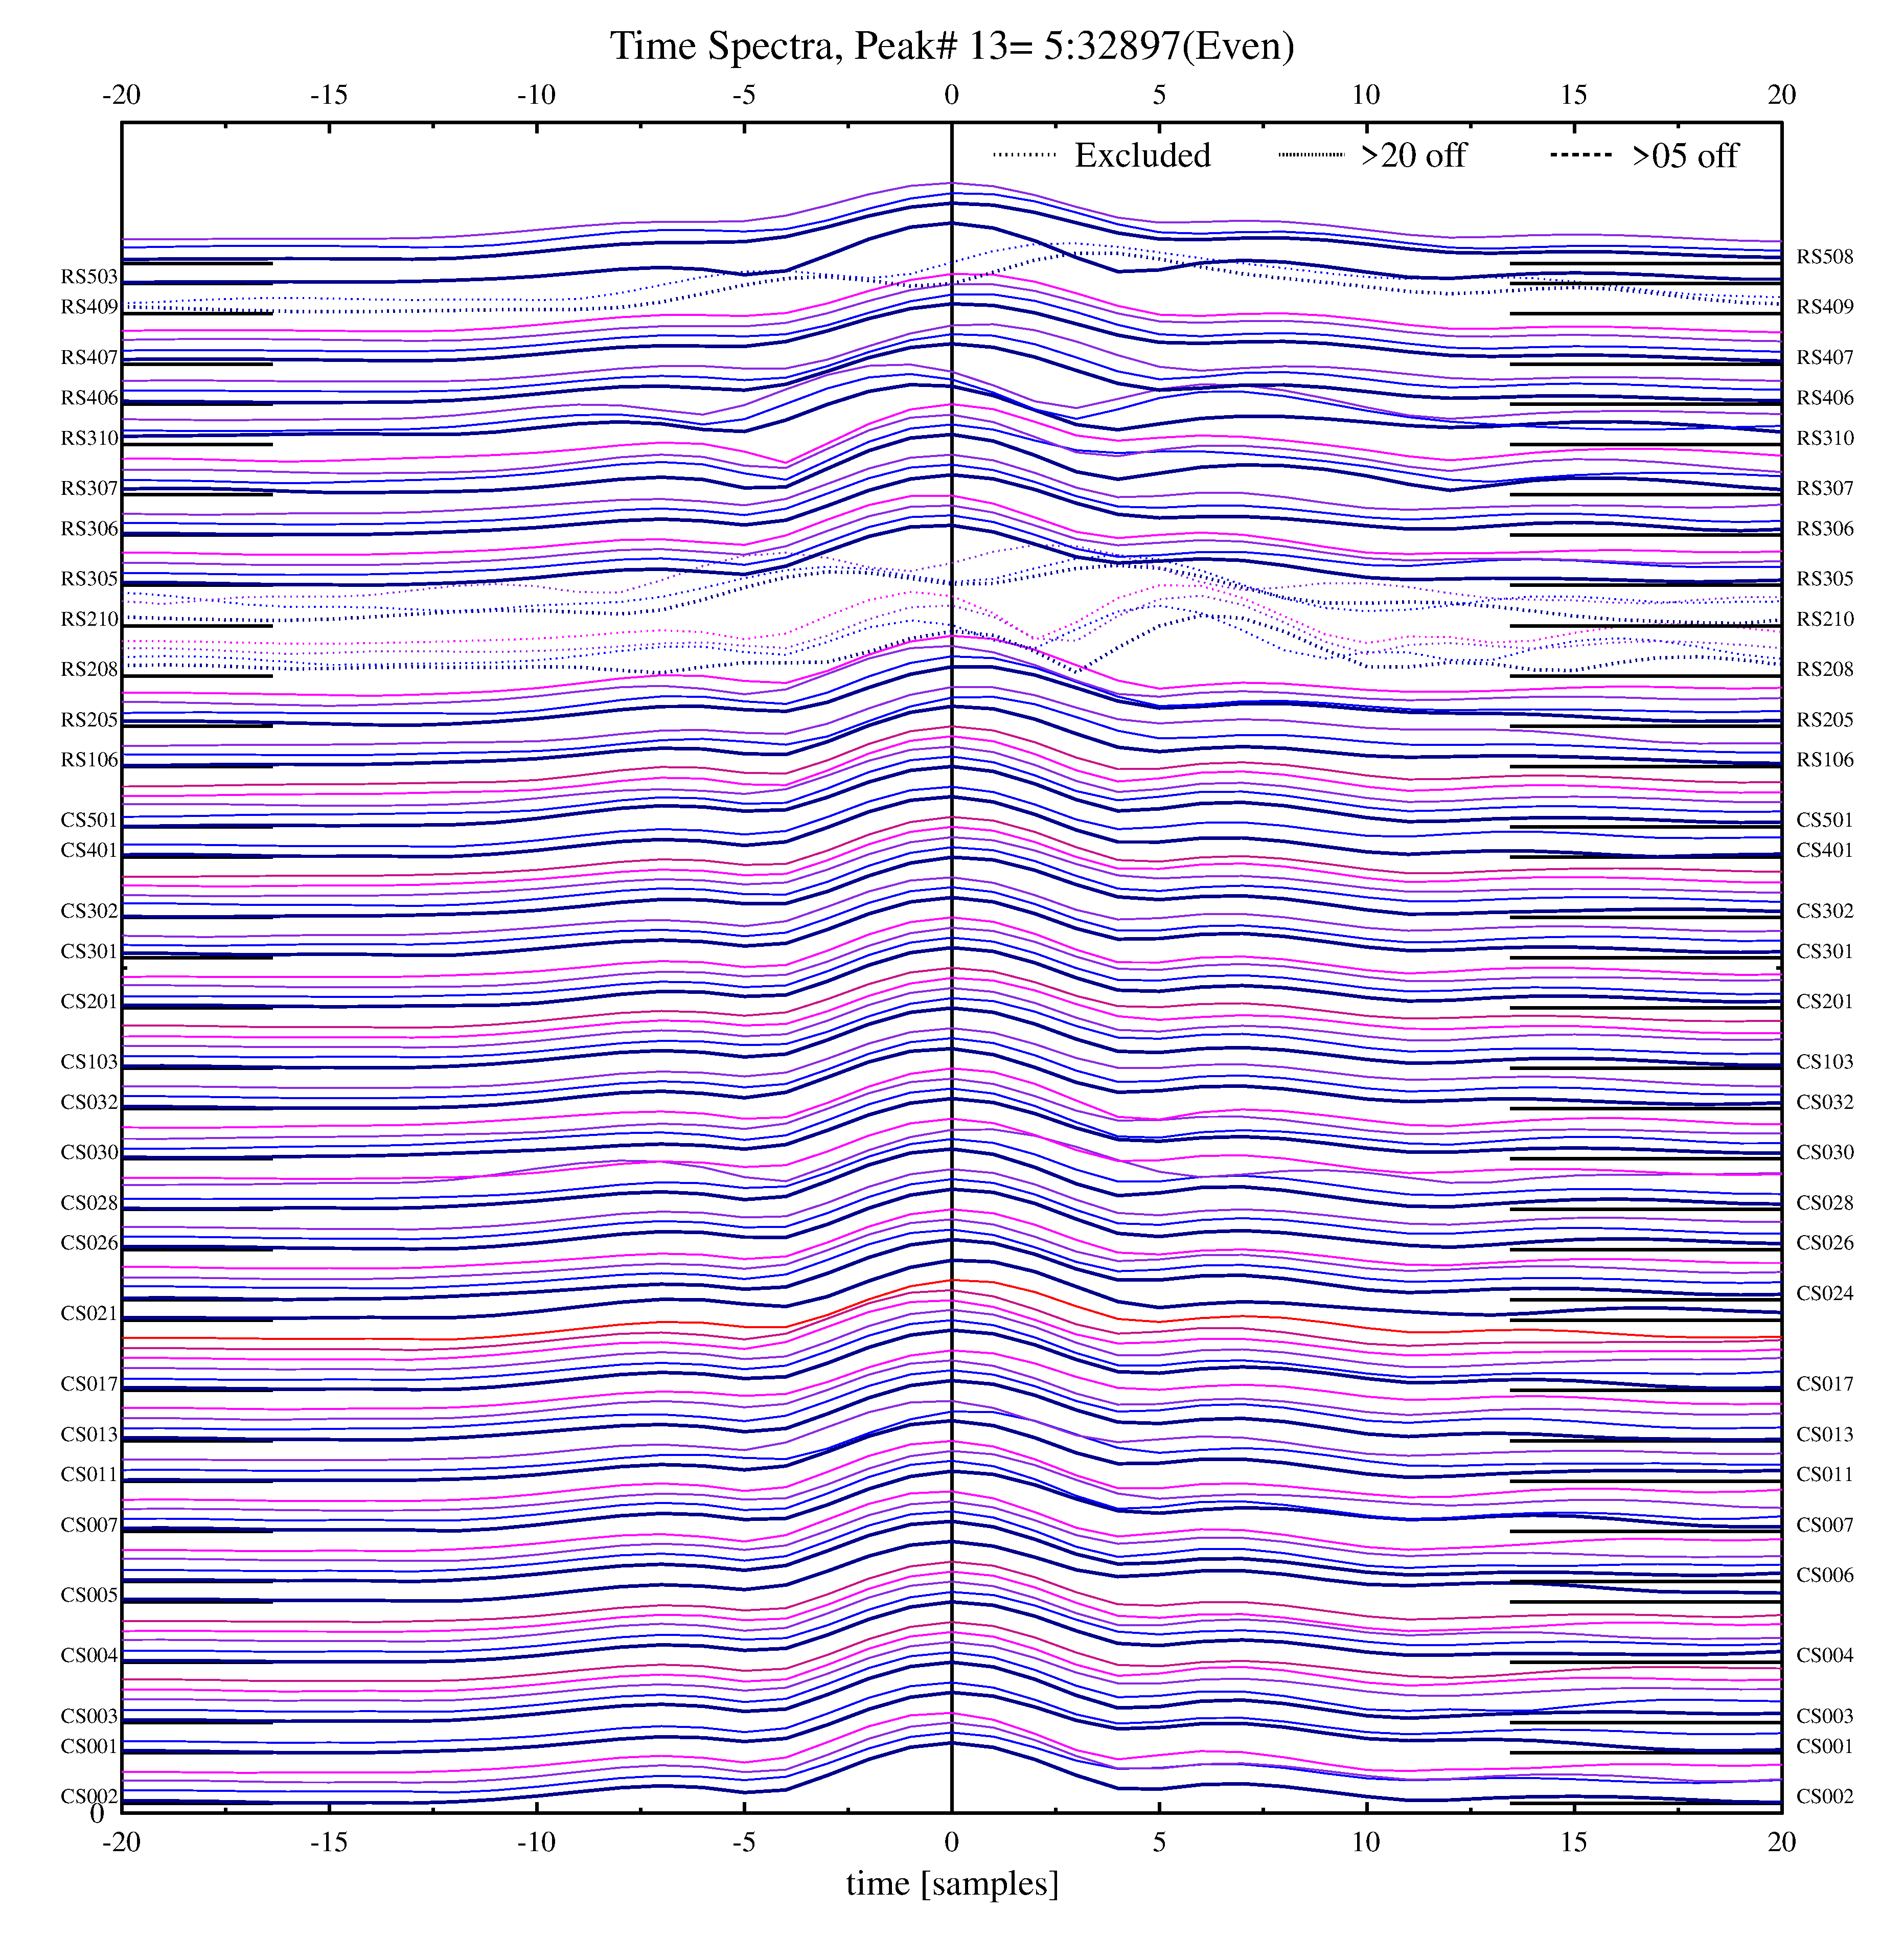
\includegraphics[width=0.69\textwidth]{Figs/XCP_13-18D1} }
%\centering{\includegraphics[ bb=1.0cm 2.4cm 24.5cm 25.7cm,clip, width=0.49\textwidth]{../Figs/SE20A7-NPMx_1HIntfSpecSel} }
	\caption{A plot of the absolute cross correlations for source \#13 for a typical flash.}	 \figlab{Cal-XCor}
\end{figure}

In \figref{Cal-XCor} a typical plot is shown of the cross correlations. The peak-time of these is used for calculating the arrival times differences that are fitted to obtain source positions. We usually work with the absolute magnitude as this yields better convergence than working with the real part. The real part has many oscillations which creates many local minima in a chi-square search, even though the position of the maximum can be determined more accurately. There is an option to plot the real parts.

For each antenna the Hilbert envelope is shown. The labels on the side helps to distinguish the different stations. Results are given in separate plots for even and odd numbered antennas. When all lines look alike, the result is good. Antennas, and stations should be excluded when the structure differs from that for the other antennas. The results for excluded stations is given by the dotted curves. It can be seen that for the case in \figref{Cal-XCor} most of them show a different structure. On the basis of these plots it may be decided to include a previously excluded station again in the fit. The paradigm is: the more the merrier, i.e.\ generally the results for the antenna calibrations are better if more stations are included, however, if for some of these station the pulse if unclear it could be that pulses from two different sources happen to arrive simultaneously in a particular antenna, the result improves if the -obviously- erroneous result is excluded. The art is to find the optimum between these conflicting requirements.


\clearpage
\subsubsection{Print output}\seclab{PrintOut}

Part a typical output (the .out file) that contains the most useful info for further processing is:

\begin{linenumbers}
\tiny
\resetlinenumber
\begin{verbatim}

i_Peak= 9 0, PeakPos=  16250, Chi^2/DegrF=   2.51   2.51, source position:   -2141.69,  -22721.36,    3935.67, RefAntTimeErr:  0.706
Stat Nr = CS001; CS002; CS003; CS004; CS005; CS006; CS007; CS011; CS013; CS017; CS021; CS024; CS026; CS028; CS030; CS032; CS103; RS106; CS201; RS208; RS210; CS301; CS302; RS305; RS306; RS307; RS310; CS401; RS406; RS407; RS409; CS501; RS503; RS508; -----
Dropped#=  0/ 5;  0/ 4;  0/ 4;  0/ 3;  0/ 2;  0/ 3;  0/ 4;  0/ 3;  0/ 6;  0/ 4;  0/ 2;  0/ 4;  0/ 5;  0/ 5;  0/ 4;  0/ 4;  0/ 5;  0/ 2;  0/ 4;  0/ 4;  0/ 3;  0/ 4;  0/ 5;  0/ 2;  0/ 3;  0/ 5;  0/ 4;  0/ 1;  0/ 1;  0/ 5;  0/ 1;  0/ 5;  0/ 4;  0/ 3; -----
RMS [ns]=   1.2;   0.6;   0.6;   0.8;   0.2;   0.4;   0.8;   1.0;   1.3;   0.7;   0.4;   0.5;   1.0;   0.9;   0.8;   0.5;   1.3;   0.9;   1.3;   2.4;   2.7;   0.4;   0.8;   0.6;   0.6;   3.5;   2.7;   0.5;   7.0;   2.6;   2.4;   0.5;   0.4;   2.3; -----
Avrg[ns]=   1.0;  -0.3;   0.5;   0.8;   0.1;  -0.3;   0.5;   1.0;   1.0;   0.5;   0.4;   0.3;   0.8;   0.4;   0.8;   0.3;   1.1;   0.5;   1.3;  -2.3;  -2.3;   0.3;   0.7;  -0.5;  -0.5;  -3.3;   2.0;   0.5;  -7.0;  -2.6;   2.4;   0.4;  -0.2;  -2.1; -----
RMS(Jac)=  0.06;  0.00;  0.02;  0.01;  0.02;  0.01;  0.01;  0.02;  0.05;  0.01;  0.05;  0.12;  0.02;  0.16;  0.13;  0.04;  0.04;  0.58;  0.05;  2.77;  4.06;  0.15;  0.21;  0.31;  0.56;  2.83;  6.46;  0.03;  2.10;  2.62;  6.03;  0.18;  0.51;  2.72;-----
\end{verbatim}
\end{linenumbers}

There is such a section for each peak. the ones towards the end of the output are for the last fits. This list for each station 1) the number of antennas that are dropped all together, because that one showed an unreasonably large difference; 2)the contribution to the RMS, 3) the mean time difference. If this matches (in absolute magnitude) the RMS for this station, then all antennas shaw about the same difference, if not, one of the antennas differs considerably. the last line shows the importance of this station for pinning down the source location.

Towards the end the following can be found

\begin{linenumbers}
\tiny
\resetlinenumber
\begin{verbatim}


C 6 1 2   18841 -72112.37,  21167.93,   5397.60,    0.00;   1.63,   1.67 RS406 RS509
exclude   RS406 RS509
C 7 0 3   27662  -6112.90, -28762.40,   6490.86,   -0.39;   1.80,   1.80
C 8 1 3   27662  -6112.90, -28762.40,   6490.86,   -0.37;   2.38,   2.50 RS208 RS210 RS310
exclude   RS208 RS210 RS310
C 9 0 4   16250  -2141.69, -22721.36,   3935.67,    0.71;   1.58,   1.58
\end{verbatim}
\end{linenumbers}

which follows the same formatting as the list needed in the input. With cut-and-paste it can thus be used conveniently. Per pulse it lists the fitted position and the value of the sqrt(chi-square) (last numbers) for this source. For a good result these numbers should not exceed 2 by much (units are nanoseconds). if the number is large, it should be searched which station is responsible for this, either by checking the listing for the pulse (see previous discussion) and/or checking the curtain and/or the cross correlation plots. This is the most tedious part of the calibration runs.

When the option \verb#" FullAntFitPrn=.true."# is switched on there is for each peak and each antenna, ordered per station, a list of the time differences between determined arrival times and calculated ones, i.e.\ the pull values for calculating the chi-square. On the basis of this information is may be decided to label a particular antenna as 'bad'. 